\section{Introduction}
\label{sec:intro}

{\em Hardware resource disaggregation} is a solution that decomposes full-blown, general-purpose servers into segregated, network-attached hardware resource pools, each of which can be built, managed, and scaled independently. With disaggregation, different resources can be allocated from any device in their corresponding pools, exposing vast amounts of resources to applications and at the same time improving resource utilization. Disaggregation also allows data-center providers to independently deploy, manage, and scale different types of resources.
Because of these benefits, disaggregation has gained significant traction from both academia~\cite{LegoOS,FireBox-FASTKeynote,ATC20-pDPM,Nitu18-EUROSYS,DDC-hotcloud20,aifm-osdi20,semeru,kona,infiniswap,fastswap} and industry~\cite{HP-TheMachine,IntelRackScale,alibaba-polardb,facebook-disaggregation,SnowFlake-NSDI20}.
%Existing disaggregated systems have focused on separating three types of resources: compute~\cite{LegoOS,disagg-gpu}, memory (or persistent memory)~\cite{LegoOS,HP-TheMachine,Lim09-disaggregate,remote-region-atc18,ATC20-pDPM,semeru,infiniswap,fastswap,hotpot-socc17}, and storage~\cite{PolarFS-VLDB18,SnowFlake-NSDI20,hailstorm-asplos20,ana-eurosys16}.
%These efforts have seen real success, and more data centers have started to adopt disaggregation at the production-scale~\cite{Ali-SinglesDay}.
%For example, Alibaba listed their disaggregated storage solution as a key enabling factor of serving 544,000 orders per second during their shopping festival~\cite{Ali-SinglesDay}.

While increasing amounts of effort go into disaggregating compute~\cite{LegoOS,disagg-gpu}, memory (or persistent memory)~\cite{LegoOS,HP-TheMachine,Lim09-disaggregate,remote-region-atc18,ATC20-pDPM,semeru,infiniswap,fastswap,hotpot-socc17}, and storage~\cite{PolarFS-VLDB18,SnowFlake-NSDI20,hailstorm-asplos20,ana-eurosys16,gimbal}, the fourth major resource, \textit{network}, has been completely left out.
At first glance, ``network'' cannot be disaggregated from either a traditional monolithic server or a disaggregated device (in this paper collectively called {\em endpoints}), as they both need to be attached to the network.        
%To answer this question, we explore the minimal network functionalities an endpoint needs to have for its connectivity.
%\bolditpara{Proposal: what can be disaggregated?}
However, we observe that even though endpoints need basic connectivity, it is not necessary to run {\em network-related tasks} at the endpoints.
These network tasks, or {\em \nt}s, include the transport layer and all high-level layers such as network virtualization, packet filtering and encryption, and application-specific functions.
%everything including and above the transport layer can 
%each endpoint only needs to manage the connectivity and reliability of the {\em last hop} --- between the endpoint to its direct connection point, and thus only needs a link layer that can handle problems happening within the last hop.
%\noteys{the above reasoning does not make sense to me. we don't have enough context to setup "last hop".}
%Everything else can be disaggregated, including a transport layer for reliable end-to-end delivery, network functions like packet filtering and network virtualization, and application-specific functionalities such as data caching. We collectively call all these ``detachable'' functionalities {\em network tasks}, or {\em \nt}s.

This paper, for the first time, proposes the concept of {\em network disaggregation} and builds a real disaggregated network system to segregate \nt{}s from endpoints.
%systematically answers a set of key questions in network disaggregation.

%\bolditpara{Proposal: disaggregated network resource pool.}
At the core of our network-disaggregation proposal is the concept of a rack-scale disaggregated {\em network resource pool}, which consists of a set of hardware devices that can execute \nt{}s and collectively provide ``network'' as a service (Figure~\ref{fig-topology}), similar to how today's disaggregated storage pool provides data storage service to compute nodes. 
Endpoints can offload (\ie, disaggregate) part or all of their \nt{}s to the network resource pool.
After \nt{}s are disaggregated, we further propose to {\em consolidate} them by aggregating a rack's endpoint \nt{}s onto a small set of network devices.
%\notearvind{might need to generalize to a network pool}
%, thereby reducing the total number of network .

We foresee two architectures of the network resource pool within a rack. The first architecture inserts a network pool between endpoints and the ToR switch by attaching a small set of endpoints to one network device, which is then connected to the ToR switch (Figure~\ref{fig-topology} (a)). The second architecture attaches the pool of network devices to the ToR switch, which then connects to all the endpoints (Figure~\ref{fig-topology} (b)). 

%\bolditpara{Motivating: what are the potential benefits of disaggregating and consolidating \nt{}s?}
%Same as disaggregating other resources like storage, 
Network disaggregation and consolidation have several key benefits.
(1) Disaggregating \nt{}s into a separate pool allows data center providers to build and manage network functionalities only at one place instead of at each endpoint. 
This is especially helpful for heterogeneous disaggregated clusters where a full network stack would otherwise need to be developed and customized for each type of endpoint.
(2) Disaggregating \nt{}s into a separate pool allows the {\em independent scaling} of hardware resources used for network functionalities without the need to change endpoints.
(3) Each endpoint can use more network resources than what can traditionally fit in a single NIC. 
(4) With \nt\ consolidation, the total number of network devices can be reduced, allowing a rack to host more endpoints.
%The final and important benefit comes from consolidation.
(5) The network pool only needs to provision hardware resources for the peak \textit{aggregated} bandwidth in a rack instead of each endpoint provisioning for its own peak, reducing the overall CapEx cost.

%Several industry products are already adopting similar architectures, \eg, multi-host NIC~\cite{bluefield} (for the first architecture) and NIC-enhanced programmable switches~\cite{arubacx10000} (for the second architecture).
%\note{I'm confused on why the ToR has to be a smart/programmable switch, not made clear in it's explanation in first half of paragraph}.
%Network disaggregation would be a new usage case of these architectures. However, it requires new features that no existing systems fully support.
Before these benefits can be exploited in a real data center, network disaggregation needs to first meet several goals, which no existing solutions fully support (see \S\ref{sec:related}).

{
\begin{figure}
\begin{center}
\centerline{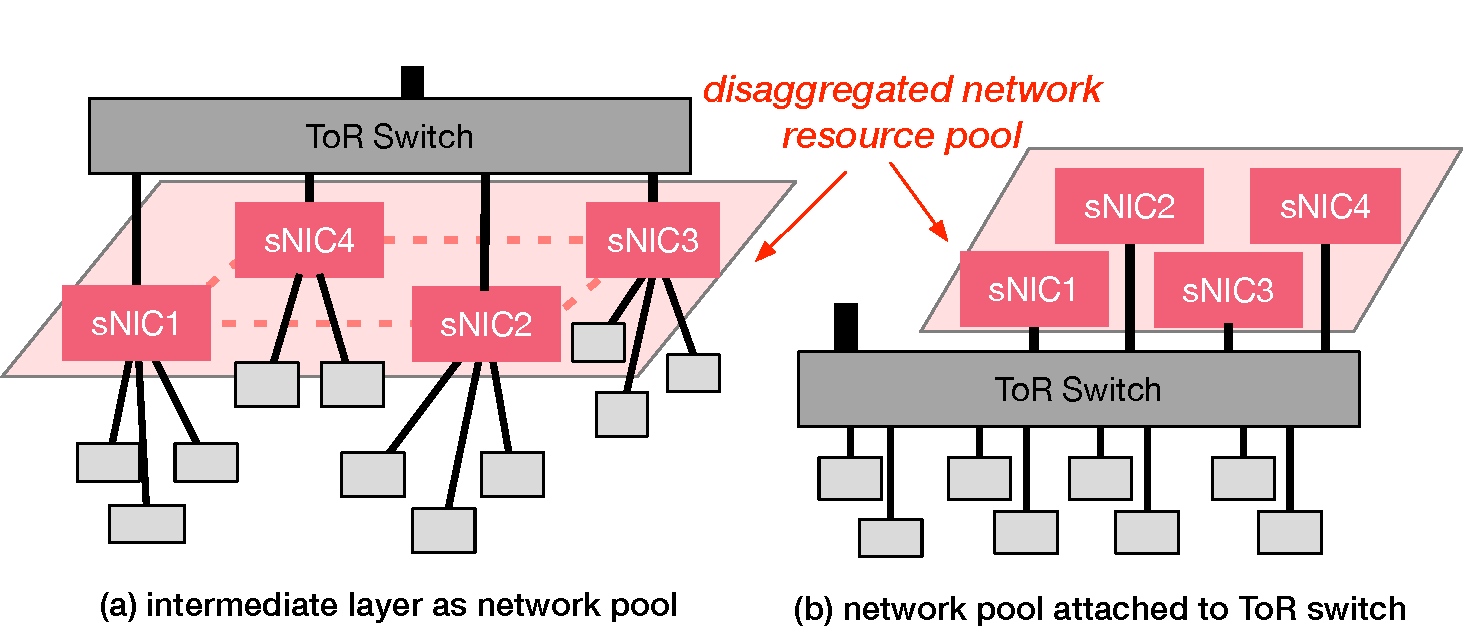
\includegraphics[width=\columnwidth]{Figures/fig-topology.pdf}}
\vspace{-0.1in}
\mycaption{fig-topology}{Overall Architectures of \sysname.}
{
Two ways of connecting \snic{}s to form a disaggregated network resource pool. In (a), dashed lines represent links that are optional.
%\yizhou{can we use another color set for this fig?}
}
\end{center}
\vspace{-0.2in}
\end{figure}
}


%\bolditpara{Building: what are the key requirements of network disaggregation and consolidation?}
First, each disaggregated network device should meet endpoints' original performance goals even when handling a much larger (aggregated) load than what each endpoint traditionally handles.
The aggregated load will also likely require many different \nt{}s, ranging from transports to application-specific functionalities.
Moreover, after aggregating traffic, there are likely more load spikes (each coming from a different endpoint) that the device needs to handle.

Second, using a disaggregated network pool should reduce the total cost of a cluster. This means that each disaggregated network device should provision the right amount of hardware resources (CapEx) and use as little of them as needed at run time (OpEx). At the same time, the remaining part of a rack (\eg, endpoints, ToR switch, cables) needs to be carefully designed to be low cost.

Third, as we are consolidating \nt{}s from multiple endpoints, in a multi-tenant environment, there would be more entities that need to be isolated. We should ensure that they fairly and safely share various hardware resources in a disaggregated network pool. 

Finally, network devices in a pool need to work together so that lightly loaded devices can handle traffic for other devices that are overloaded.
This load balancing would allow each device to provision less hardware resources as long as the entire pool can handle the peak aggregated load of the rack.

%key challenges consolidation
%sharing, autoscaling, dist
%control plane scalability

Meeting these requirements together is not easy as they imply that the disaggregated network devices need to use minimal and properly isolated hardware resources to handle large loads with high variation, while achieving application performance as if there is no disaggregation.

To tackle these challenges and to demonstrate the feasibility of network disaggregation, we built \textit{\textbf{SuperNIC}} (or \textit{\snic} for short), a new hardware-based programmable network device designed for network disaggregation.
%why new hardware-based sNIC. functions like transport need high speed parallel processing, and software is too slow for that. however, traditional NIC hardware or hardware-based SmartNIC does not offer the autoscaling or fair sharing feature we need for consolidation.
An \snic\ device consists of an ASIC for fixed systems logic, FPGA for running and reconfiguring \nt{}s, and software cores for executing the control plane.
We further built a distributed \snic\ platform that serves as a disaggregated network pool.
Users can deploy a single \nt\ written for FPGA or a directed acyclic graph (DAG) execution plan of \nt{}s to the pool.

To tightly \textbf{consolidate} \nt{}s within an \snic, we support three types of resource sharing: (1) splitting an \snic's hardware resources across different \nt{}s ({\em space sharing}), (2) allowing multiple applications to use the same \nt{} at different times ({\em time sharing}), and (3) configuring the same hardware resources to run different \nt{}s at different times ({\em time sharing with context switching}).
For space sharing, we partition the FPGA space into {\em region}s, with each hosting one or more \nt{}s.
Each region could be individually {\em reconfigured} (via FPGA partial reconfiguration, or {\em PR}) for starting new \nt{}s or to context switch \nt{}s.
Different from traditional software systems, hardware context switching with PR is orders of magnitude slower, which could potentially impact application performance significantly.
To solve this unique challenge, we propose a set of policies and mechanisms to reduce the need to perform PR or to move it off the performance-critical path, \eg, by keeping de-scheduled \nt{}s around like a traditional victim cache, by not over-reacting to load spikes, and by utilizing other \snic{}s when one \snic\ is overloaded.
%\notearvind{Might be worth saying that we also rely on other sNICs' resources if a local sNIC is overloaded.}

To achieve high \textbf{performance} under large, varying load with minimal cost, we automatically scale (auto-scale) an \nt{} by adding/removing instances of it and sending different flows in an application across these instances.
%\noteyiying{@Yizhou, do we send different flows to different instances or it's packet level? --- YS: We use flows. We cannot do individual packet LB, because there are states associated with each flow.}
We further launch different \nt{}s belonging to the same application in parallel and send forked packets to them in parallel for faster processing.
%We achieve high throughput using two levels of parallelism:
%{\em \nt{} parallelism} where a packet goes through multiple \nt{}s in parallel and {\em instance parallelism} where we launch multiple instances of the same \nt{} to handle different packets in an application.
%Apart from the above data-plane designs, we build a scalable control plane.
%To achieve low scheduling latency and scalability, we 
%propose a scheduler that centers around a new notion, {\em \nt\ chaining}.
%The idea is to 
To achieve low scheduling latency and improve scalability, we group \nt{}s that are likely to be executed in a sequence into a chain.
% and to have our central scheduler schedule packets only once for the entire chain. 
Our scheduler reserves credits for the entire chain as much as possible so that packets execute the chain as a whole without involving the scheduler in between.
%Doing so improves both packet-processing latency and scheduler scalability.

To provide \textbf{fairness}, we adopt a fine-grained approach that treats each internal hardware resource separately, \eg, ingress/egress bandwidth, internal bandwidth of each shared \nt, payload buffer space, and on-board memory, as doing so allows a higher degree of consolidation.
%Our context is unique in that the packet processing system itself requires multi-dimensional resource sharing. 
We adopt Dominant Resource Fairness (DRF)~\cite{DRF} for this multi-dimensional resource sharing.
%For the first time in networking systems, we consider multi-dimensional resource sharing and provide Dominant Resource Fairness (DRF)~\cite{DRF}. 
Instead of user-supplied, static per-resource demands as in traditional DRF systems, we monitor the actual load demands at run time and use them as the target in the DRF algorithm.
Furthermore, we propose to use ingress bandwidth throttling to control the allocation of other types of resources.
We also build a simple virtual memory system to \textbf{isolate and protect} accesses to on-board memory. %All \nt's memory accesses use 

Finally, for \textbf{distributed \snic{}s}, we automatically scale out \nt{}s beyond a single \snic\ when load increases and support different mechanisms for balancing loads across \snic{}s depending on the network pool architectures.
For example, with the switch-attached pool architecture, we use the ToR switch to balance all traffic across \snic{}s.
With the intermediate pool architecture, we further support a peer-to-peer, \snic-initiated load migration when one \snic\ is overloaded.

\if 0
When one \snic\ is overloaded and needs to accommodate too much network bandwidth, on-chip hardware resources, or off-chip memory space, traditional solutions would drop packets/\nt{}s or provision more hardware resources. The former impacts application performance, and the latter results in resource wastage when loads are not at their peaks. 
Our idea is to utilize other \snic{}s to handle load spikes, based on the observation that not all \snic{}s under a rack would run at their peak load at the same time. Essentially, with distributed \snic{}s, we provision for the maximum aggregated bandwidth in a rack instead of the sum of peak loads under each \snic.
Specifically, to support overloaded network bandwidth or on-chip hardware resources at an \snic, we create an \nt\ at another \snic\ that has a lighter load. 
The current \snic\ then only serves as a simple pass-through device to redirect packets to the new \snic.
%, with the latter sending packets to the next hop after processing them.
To support overloaded memory space at an \snic, our virtual memory system transparently swaps memory to/from an \snic{} with less memory pressure.
\fi

{
\begin{figure*}
\begin{minipage}{0.25\textwidth}
\begin{center}
\centerline{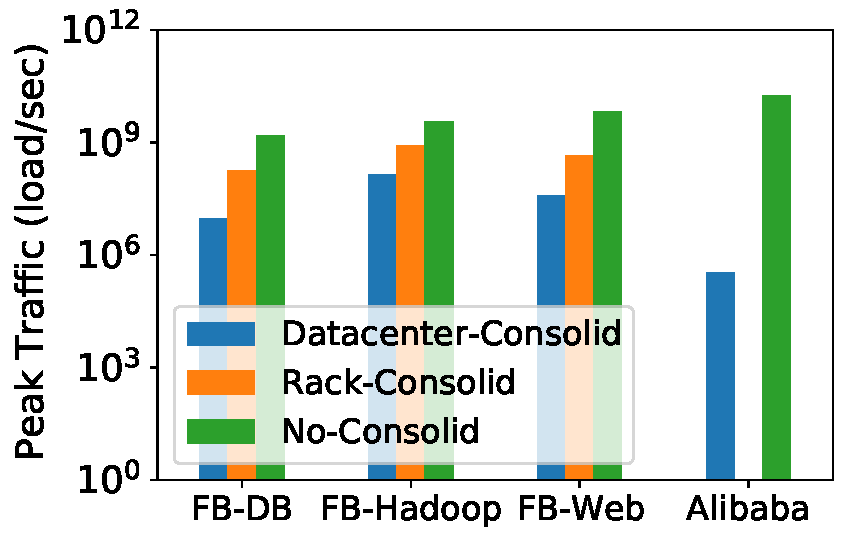
\includegraphics[width=\textwidth]{Figures/fig_fb_alibaba_trace.pdf}}
\vspace{-0.1in}
\mycaption{fig-fb-alibaba}{Consolidation Analysis of Facebook and Alibaba Traces.}
{
Load represent relative amount and have different units for FB and Alibaba.
}
\end{center}
\end{minipage}
\begin{minipage}{0.25\textwidth}
\begin{center}
\centerline{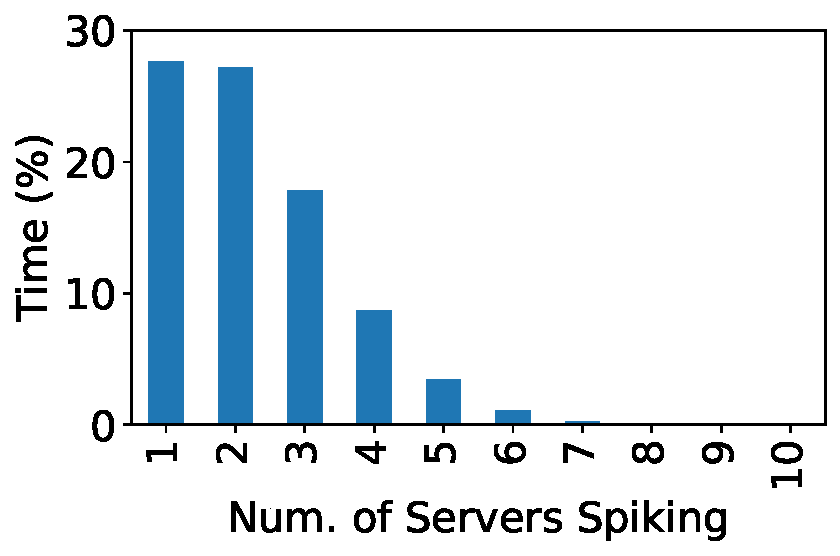
\includegraphics[width=\textwidth]{Figures/spike-trace-analysis.pdf}}
\vspace{-0.1in}
\mycaption{fig-spike-var}{Load Spike Variation across Endhosts in FB.}
{
}
\end{center}
\end{minipage}
\begin{minipage}{0.5\textwidth}
\begin{center}
\centerline{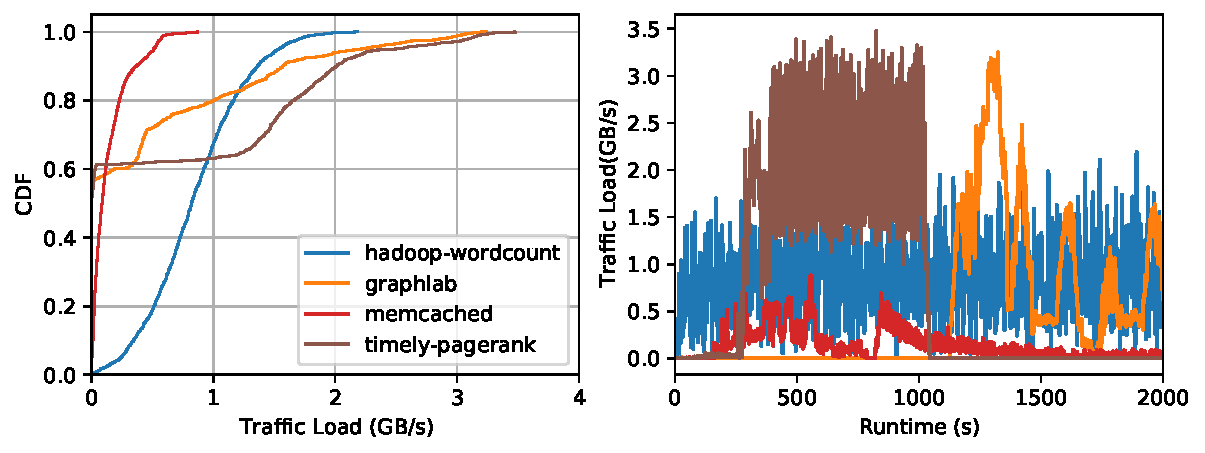
\includegraphics[width=\textwidth]{Figures/fig-osdi16-net-trace.pdf}}
\vspace{-0.15in}
\mycaption{fig-OSDI16NetTrace}{Network traffic for accessing disaggregated memory.}
{
}
\end{center}
\end{minipage}
\vspace{-0.15in}
\end{figure*}
}



We prototype \snic\ with FPGA using two 100\Gbps, multi-port HiTech Global HTG-9200 boards~\cite{htg9200}.
%The data plane runs on FPGA directly, while the control plane runs in software cores deployed on FPGA.
We build three types of \nt{}s to run on \snic:
reliable transport, traditional network functions, and application-specific tasks, and port two end-to-end use cases to \snic.
The first use case is a key-value store we built on top of real disaggregated memory devices~\cite{Clio}.
We explore using \snic{}s for traditional \nt{}s like the transport layer and customized \nt{}s like key-value data replication and caching.
%For the latter, the client only needs to send one copy to the \snic, which will send copies of the data to multiple memory devices.
%customized network abstraction for disaggregated memory device: a key-value store interface (rather than the standard messaging interface).
%Furthermore, we 
The second use case is a Virtual Private Cloud application we built on top of regular servers by connecting \snic{}s at both the sender and the receiver side.
We disaggregate \nt{}s like encapsulation, firewall, and encryption to the \snic{}s.
%a go-back-N reliable transport; a set of network functions including firewall, AES encryption, and VPN Gateway; and a set of application-specific functions including key-value store replication and caching.
We evaluate \snic\ and the ported applications with micro- and macro-benchmarks and compare \snic\ with no network disaggregation and disaggregation using alternative solutions such as multi-host NICs and a recent multi-tenant SmartNIC~\cite{panic-osdi20}.
Overall, \snic\ achieves 52\% to 56\% CapEx and OpEx cost savings with only 4\% performance overhead compared to a traditional non-disaggregated per-endpoint SmartNIC scenario.
%Our results running a Facebook key-value trace~\cite{Atikoglu12-SIGMETRICS} show that \snic's consolidation of four endhosts and two \nt{}s saves 64\% costs compared to no consolidation, with only 1.3\% performance overhead.
Furthermore, the customized key-value store caching and replication functionalities on \snic\ improves throughput by 1.31\x\ to 3.88\x\ and latency by 1.21\x\ to 1.37\x\ when compared to today's remote memory systems with no \snic.
%We will open source \snic\ upon the publication of this paper.





\if 0
There is a trend in disaggregating datacenters,
in which monolithic servers are segregated into cpu, memory, disk
resource pools and connected to the network directly.
Disaggregation makes it easy to manage and scale each resource pool independently.
While increasing amount of effort go into disaggregating compute,
memory, and storage, the fourth major resource in datacenter, network,
has been completely left out. No work has attempted to disaggregate the network.
At first glance, network cannot be disaggregated from either
a traditional monolithic server or a disaggregated device, as
they both need to be attached to the network
and each endpoint is provisioned with its own network interface (i.e., NIC)
and the associated network stack. This raises the question:

\textit{Should we and how can we disaggregate the network?}

We answer this question in the affirmative:
we should disaggregate and then consolidate the network.
In our preliminary study,
we find both regular server and disaggregated clusters have bursty network traffic
while the networking resource is highly under-utilized.
The root cause is that network is tightly coupled with
other resources (e.g., compute or memory) and hence,
making it impossible to
provision the right amount of networking resource for individual endpoints.
Similar to traditional disaggregation,
if we can disaggregate the networking resource and further
aggregate them into a network resource pool,
it could enjoy easier management, scaling, and resource packing.
We envision this is applicable and beneficial
for two types of endpoints: regular monolithic servers
and disaggregated devices.

We propose to \textit{disaggregate} network functionalities
from individual endpoints in a rack
and \textit{consolidate} them into a \textbf{\textit{network resource pool}}.
%
Crucially, the consolidation enables statistical multiplexing of resources that
allows us to move away from provisioning for peak utilization
on a per-node basis to provisioning for the
expected peak utilization for a cluster of nodes.
Also, consolidating network functionalities into a separate
pool makes it easy for datacenter operators to manage them.
%
Three types of network functionalities are moved:
\textit{1)} packet processing logic in NIC hardware,
\textit{2)} software network stacking running at host CPU,
and \textit{3)} advanced application-specific network functions.
%
As a result, individual endpoints no longer need to provision
hardware and software resources for networking,
they can directly use services exposed by the network resource pool.
%
In other words, the network resource pool essentially provides
\textbf{\textit{network-as-a-service}} to the rest of the datacenter.


Network disaggregation and consolidation presents several new challenges.
%
First, network has always been an integral part for any computer systems design.
Hence, it is challenging to extract the network functions
while ensuring correctness and performance.
%
Second, a key question is how to implement the network resource pool.
In order to meet the goals of disaggregation,
the pool must be flexible, power-efficient, high-performance, easy to manage, and secure.
Disaggregated datacenter poses several unique challenges
like the exploded number of network ports and the mix of heterogeneous devices
\fi



\if 0
In this paper, we will focus on the second challenge.
We take a detailed survey on all emerging network devices
and evaluate whether they are qualified to make the network resource pool.
In specific, we review
\textit{programmable switch}~\cite{netcache-sosp17,incbricks-asplos17,distcache-fast19,pegasus-osdi20,hpcc-sigcomm19,netlock-sigcomm20,cheetah-sigmod20,racksched-osdi20,tea-sigcomm20},
\textit{circuit switch}~\cite{helios-sigcomm10,mordia-sigcomm13,reactor-nsdi14,rotornet-sigcomm17,sirius-sigcomm20,dRedBox-DATE,shoal-nsdi19},
\textit{coherent fabrics}~\cite{GenZ,OpenCAPI,CCIX,CXL},
\textit{middleboxes}~\cite{walfish-osdi04,comb-nsdi12,aplomb-sigcomm20},
\textit{NFV}~\cite{clickos-nsdi14,e2,netbricks,resq-nsdi18,metron-nsdi18,flowblaze-nsdi19,panic-osdi20,azure-nsdi18},
and \textit{multi-host NICs}~\cite{Intel-RedRockCanyon,Mellanox-Multihost}.

After a rigorous examination, we find none of them meets all our goals.
In response, we propose \sysname, a new network device specifically
designed for network disaggregation and consolidation.
A set of SuperNICs make a disaggregated network resource pool,
which sits in between endpoints and a ToR switch.
All the SuperNICs are connected together through a ring or a torus (see Figure~\ref{fig-topology}).
We expect it to have high performance, flexible abstractions,
safe and efficient consolidation, adaptive scaling, and failure handling.


Overall, our contributions are:
\begin{itemize}
\vspace{-0.05in}
\item To the best of our knowledge, we are the first to
disaggregate and consolidate network in datacenters.
\vspace{-0.05in}
\item We review various emerging networking devices.
\vspace{-0.05in}
\item We propose SuperNIC, a new device specifically tailored for network disaggregation and consolidation.
\end{itemize}

\fi

